\documentclass[%
reprint,nofootinbib,
amsmath,amssymb,
aps,
]{revtex4-1}
\usepackage{graphicx}% Include figure files
\usepackage{dcolumn}% Align table columns on decimal point
\usepackage{bm}% bold math
\usepackage[utf8]{inputenc}
\usepackage{listings}
\usepackage{amsmath}
\usepackage{physics}
\usepackage{booktabs}
\usepackage{float}
\usepackage[bottom]{footmisc}
\usepackage{scrextend}
\bgroup
\def\arraystretch{1.3}
\newcommand{\HRule}{\rule{\textwidth}{0.5mm}}
\makeatletter
\newcommand*{\rom}[1]{\expandafter\@slowromancap\romannumeral #1@}
\makeatother

\begin{document}
\onecolumngrid

\begin{center}
	\large\textbf{Methods of numerical integration\\ \small{The Gaussian Quadrature and Monte Carlo Procedures}}
\end{center}
\vspace{5mm}

\begin{center}
	\small{$^1$ Oline A. Ranum}\\
\end{center}

\begin{center}
	\small{$^1$ University of Oslo, Institute of physics, 
		olinear@student.matnat.uio.no}
\end{center}

\begin{center}
	\textit{\today}
\end{center}
\vspace{7mm}
\noindent 
\HRule \vspace{2mm}\\
The main objective of this paper is to evaluate the efficiency and accuracy of Monte Carlo Integration compared to the Gauss-Legendre and Gauss-Laguerre quadrature. As such, the procedures are employed to preform numerical integration yielding the expectation value of the ground state correlation energy, $E[f]$, between two electrons in an helium atom. The Gauss-Legendre procedure results in $E[f] \approx (1.9 \pm 0.2)\times 10^{-1}$ for $N=27$. The Gauss-Laguerre procedure yields $E[f]\approx (1.9 \pm 0.1)\times 10^{-1}$ for $N=15$. The accuracy is based on the relative error, which is considered to be a poor method for approaching the error although a more elaborate error analysis is left for future work. The best result from brute force Monte Carlo integration using a uniform distribution function is found for $N=10^7$, yielding $E[f]\approx (1.8983 \pm 0.0003)\times 10^{-1}$. The Monte Carlo estimate is improved by implementing the concept of importance sampling, yielding a result of $E[f]\approx (1.9292 \pm 0.0004)\times 10^{-1}$ using an exponential distribution function. The accuracy estimate is given as the variance for the Monte Carlo estimations. In the last section of this paper the Monte Carlo integration method is parallelized to run on four processors simultaneously using MPI, giving the result $E[f]\approx (1.9264 \pm 0.0004)\times 10^{-1}$. The parallelized Monte Carlo process is found to have the greatest temporal efficiency in regards to accuracy. 
\vspace{1.5mm}  \\
\HRule
\vspace{0.3cm}

\section{Introduction}
\vspace{5mm}
\twocolumngrid \noindent
Wherever you go in science today, there is a need for approximating integrals that do not have a known closed form solution. The term numerical integration first occurred in the 20th century, and has since become one of the most valuable tools in modern science. Amongst some of the most famous approaches to numerical integration are the Gaussian Quadrature and Monte Carlo integration. The Gaussian quadrature seeks the best numerical estimate of an integral by attempting to optimize a selection of abscissas. Monte Carlo integration, on the other hand, is based on a far simpler selection of random abscissas preformed on a much larger scale. This paper intends to evaluate the efficiency of both approaches by applying the two methods to solve for a physical system where an exact solution is known. The estimate will be preformed on the expectation value of the ground state correlation energy between two electrons in an helium atom. \\
\indent The paper initially presents the theory behind the integration methods, and elaborates on how the procedures are applied to estimate the correlation energy. In the first part of the paper the integral is estimated using the Gauss-Legendre quadrature, followed by the Gauss-Laguerre quadrature. In the second part of the paper a brute force Monte Carlo integration is implemented using a uniform distribution function. The Monte Carlo approach is then improved by implementing the concept of importance sampling and by parallelization of the code. Results are presented and discussed in regards to both efficiency and accuracy. In the end a conclusion is presented on the back of the discussion. \\ \indent 
A comprehension for the foundations of numerical methods yield ground for new applications. For instance, the appreciation of Monte Carlo methods across various fields has given sciences like chemistry, physics and biology an invaluable tool. Monte Carlo methods are widely used to preform  multi-dimensional integrals across all sections of science. It even happens to gives life to new sections, like the up and coming sector of statistical finance. When compared to methods of differentiating origins, like the Gaussian quadrature, the evaluation broadens our comprehension for numerical approaches in general. Comparing alternative approaches presents the  opportunity for discussion of both efficiency and accuracy of methods. Numerical integration is a rich field that continuous to grow, and it is my hope that this paper will be a contribution to a deeper understanding of the relationship between our selected methods. \newpage 
 
\section{Theory} \noindent 
The basic idea behind all numerical integration is to approximate an integral with
\begin{equation}\label{numint}
I = \int_{a}^{b}f(x)dx \approx \sum_{i=0}^{N-1} \omega_if(x_i)
\end{equation}
where $\omega$ and $x$ are respectively the chosen weights and abscissas. 


\subsection*{The Gaussian quadrature} \noindent 
The Gaussian quadrature is based on the notion that a suitable variation of the abscissas would in general lead to a better accuracy than the traditional interpolatory quadrature rules, such as Simpson's- or the trapezoidal method. The traditional approaches preassigns the abscissas equidistantly, or with a fixed distribution, while Gaussian quadrature seeks the best numerical estimate by optimizing the choice of abscissas. The fundamental theorem of Gaussian quadrature states that this optimal choice is precisely the roots of the orthonormal polynomial of the same interval and weighting function. As stated in Kyte and Schaferkotter, the $n$-point Gaussian quadrature is optimal because it fits all polynomials up to a degree $2n-1$ exactly [Kythe \& Schaferkotter, 2005]. \\ \indent 
The Gaussian quadrature provides the freedom to choose both the weighting coefficients and the location of the abscissas at which the function is to be evaluated, leaving twice the degrees of freedom in regards to the classical interpolatory quadratures [Press et al. 2007]. As such, many variations and generalizations of the Gaussian formulas have been developed on the form of equation \ref{numint}, where the weights $\omega_i$ are positive zeros of certain orthogonal polynomials of suitable abscissas $x_i$ [Kythe \& Schaferkotter]. \\
\indent It is important to note that higher order does not necessarily imply higher accuracy. The former only implies the latter in the case where the integrand is very smooth, in the sense that the integrand is well approximated by a polynomial. In the case of a Gaussian quadrature, it is possible to arrange both weights and abscissas to make integrals exact for a class of integrands on the form of polynomials times some known function $W(x)$. One chooses $W(x)$ to remove singularities from the desired integral. I.e. given $W(x)$ and an integer N, it is possible to find a set of weights $w_j$ and nodes $x_j$ such that the approximation 
\begin{equation*}
	\int_{a}^{b}W(x)f(x)dx \approx \sum_{j = 0}^{N-1}w_jf(x_j)
\end{equation*}
is exact if $f(x)$ is a polynomial [Press et al.].

\subsubsection*{Orthonormal polynomials} \noindent 
The subject of Gaussian quadratures was extended by Jacobi's derivation of Gauss's work, by means of orthogonal polynomials. A set of polynomials $\{p_i\}$ of degree $i$ is said to be orthogonal with respect to the inner-product if $\langle p_i, p_j \rangle = 0$ for $i\not = j$ on a finite or infinite interval $[a,b]$. That is, if the powers are orthonormalized, one should obtain a unique set of polynomials $p_i(x)$ of degree $n$ such that \vspace{2mm} \\
\begin{equation*}
	\braket{p_i}{p_j} = 
	\int_{a}^{b} W(x)p_i(x)p_j(x)dx = \delta_{ij} 
\end{equation*}\vspace{2mm} \\
where $\delta_{ij}$ is the Kronecker delta\vspace{1mm} \\
\begin{equation*}
	\delta_{ij} = \left\{
	\begin{array}{ll}
	1 & i = j\\
	0 & i \not =j 
	\end{array} \right\}
\end{equation*}\vspace{1mm} \\
The orthogonality property for polynomials defined in this manner is directly translatable to discrete set of polynomials. Two functions are said to be normalized if its scalar product with itself is unity. A set of functions that are all mutually orthogonal and also all  individually normalized is called an orthonormal set [Press et al.].
\subsubsection{Constructing orthogonal polynomial sets} \noindent 
It is possible to find a set of polynomials through recurrence relations which has the property of being mutually orthogonal over a specified weight function W(x) and that includes exactly one polynomial $p_j(x)$, of order $j$. Press et al. describes the constructive procedure as following\vspace{0.5mm} \\
\begin{align*}
	p_{-1}(x) &\equiv 0\\
	p_{0}(x) &\equiv 1\\
	p_{j+1}(x) &\equiv (x-a_j)p_j(x)-b_jp_{j-1}(x)\\
\end{align*} 
where  \\
\begin{align*}
	a_j &= \dfrac{\braket{xp_j}{p_j}}{\braket{p_j}{p_j}} &\hspace{1mm} j = 0,1, \dots \\ &&\\
	b_j &=\dfrac{\braket{p_j}{p_j}}{\braket{p_{j-1}}{p_{j-1}}} &\hspace{1mm} j = 1,2, \dots
\end{align*} \vspace{0.5mm} \\
The coefficient $b_0$ would be arbitrary, and can therefore be set to zero. Then the polynomial $p_j(x)$ have exactly $j$ distinct roots in a given interval $[a,b]$. For classical orthogonal polynomials, such as the Gauss-Legendre and Gauss-Laguerre, the coefficients $a_j$ and $b_j$ have an explicit solution. Thus, the problem reduces to determining the zeros of the polynomial $p_N(x)$, and computation of the weights $w_i$ [Press et al.]

\subsubsection{Computation of abscissas and weights} \noindent
Both the Gauss-Legendre and - Laguerre are classical, well-studied, orthogonal polynomials and can be used as good starting guesses for iterative polynomial recurrence relations. After an initial guess is made, one can apply Newtons method, and expect  it to converge rather rapidly to locate zero-points. For the Gauss-Legendre and Gauss-Laguerre quadrature the following direct root finding based on the coefficients $a_j$ and $b_j$ is considered to be faster than any other method by a factor of 3 to 5\vspace{5mm}\\
\vspace{2mm} \noindent 
\textit{Gauss-Legendre}: 
\begin{align}\label{glegfunc} 
	&W(x) = 1 \hspace{3mm} -1 < x < 1 \nonumber \\ & \nonumber \\ 
	&(j+1)P_{j+1} = (2j +1)xP_j - jP_{j-1}
\end{align} 
\vspace{2mm} \\ \noindent 
\textit{Gauss-Laguerre} \vspace{2mm}
\begin{align}\label{glagfunc}
&W(x) = x^\alpha e^{-x} \hspace{3mm} 0 < x < \infty \nonumber  \\ & \nonumber \\ 
&(j+1)L_{j+1}^\alpha = (-x+2j+\alpha+1)L_j^\alpha \nonumber \\ & \hspace{35mm}-(j+\alpha)L_{j-1}^\alpha
\end{align} 
\hspace{6.8cm}[Press et al.] 
\subsubsection{The Newton-Raphson method} \noindent 
In order to employ Newtons method to locate the the appropriate abscissas, one only needs the suitable polynomial, its derivative and an initial abscissas.  The Newton-Raphson method is a one-dimensional root-finding routine, that easily generalizes to multiple dimensions. The method requires evaluation of the function and its derivative at arbitrary abscissas x, and is geometrically an extension of a tangent line at the current point $x_i$. The tangent is extended until it crosses zero, then the next guess is placed at $x_{i+1}$ to the abscissa of that zero crossing. The method derives from a Taylor series expansion of a function in the neighborhood of a point. The Newton-Raphson formula is expressed as \vspace{2mm} \\
\begin{equation*}
	x_{i+1} = x_i -\dfrac{f(x_i)}{f'(x_i)}
\end{equation*}
with associated error propagation\vspace{2mm} \\
\begin{equation}\label{newton}
	\epsilon_{i+1} = \epsilon_i  -\dfrac{f(x_i)}{f'(x_i)}
\end{equation}\vspace{2mm} \\
This method is efficient as it converges quadratically. The derivate of the polynomial can be evaluated using the standard relations in terms of $p_N$ and $p_{N-1}$ \vspace{2mm} \\
\begin{equation*}
	f'(x) \approx \dfrac{f(x+dx)- f(x)}{dx}
\end{equation*}\vspace{2mm} 
 \hspace{65mm} [Press et al.]

\subsection*{Stochastic Monte-Carlo Integration}\noindent 
Monte Carlo integration evaluates a function $f(x)$ on a randomly selected sample of abscissas $x_i$ and estimates the integral of $f(x_i)$. The fundamental theorem of Monte Carlo integration gives an estimate of the integral of the function over a multidimensional volume V\vspace{2mm} \\
\begin{equation}
	\int f dV \approx V \langle f\rangle \pm V\sqrt{\dfrac{ \langle f^2 \rangle - \langle f \rangle^2}{N}}
\end{equation}\vspace{2mm} \\
The $\pm$-term is the one standard deviation error estimate for the integral. The angle brackets denote taking the arithmetic mean over the N sample points so that \vspace{2mm} \\
\begin{equation*}
	\langle f \rangle \equiv \dfrac{1}{N}\sum_{i=0}^{N-1}f(x_i)
\end{equation*}
\begin{equation*}
\langle f^2 \rangle \equiv \dfrac{1}{N}\sum_{i=0}^{N-1}f^2(x_i)
\end{equation*}\vspace{2mm} 
\hspace{65mm}[Press et al.]

\subsubsection{Probability distribution functions}\noindent
For a broad range of Monte Carlo applications, the only requirement is that a probability distribution function (PDF) that describes the physical system is known. Once a PDF is established a Monte Carlo simulation can proceed by taking random samplings from the PDF. The result is built on the average of many simulations over the number of observations, so the variance can be predicted. The PDF is a function $p(x)$ on the domain which in the discrete case gives us the probability or relative frequency with which these values of X occur \vspace{0.5mm} \\
\begin{equation*}
	p(x) = \textnormal{Prob}(X=x)
\end{equation*}\vspace{0.5mm} \\
The PDF must satisfy two properties. First, the PDF has to be normalized so that all the probabilities add up to unity\vspace{0.5mm} \\
\begin{equation*}
	\sum_{x_i\in \mathcal{D}} p(x_i) = 1
\end{equation*} \vspace{0.5mm} \\
Secondly, assuming that the PDF is normalized, the probability has to be of a positive nature \vspace{0.5mm} \\
\begin{equation*}
	0 \leq p(x) \leq 1
\end{equation*}\vspace{0.5mm} \\
One especially important PDF is the uniform distribution\vspace{2mm} \\
\begin{equation}\label{unipdf}
	p(x) = \dfrac{1}{b-a}\Theta(x-a)\Theta(b-x)
\end{equation}\vspace{0.5mm} \\
where
\begin{align*}
	\Theta(x) &= 0& \hspace{2mm} x < 0\\
	\Theta(x) &= 1& \hspace{2mm} x \geq 0\\
\end{align*}\vspace{2mm} \\
Another important probability distribution is the exponential distribution \vspace{2mm} \\ 
\begin{equation}\label{exppdf}
	p(y) = \exp{-y}
\end{equation} \\
where $p(y)$ is given by the uniform distribution of $y\in[0,1]$. Assuming that the probability is conserved through variable transformation one finds that  \vspace{2mm}\\
\begin{equation*}
p(y)dy = \exp{-y}dy = dx
\end{equation*} \\ 
The above definition is a functions of a single stochastic variable, and is  known as univariate. A PDF consisting of multiple variables is usually referred to as multivariate, and its expectation value is defined similarly as the univariate evaluation. If all stochastic variables are taken into account simultaneously, the form of the expectation value becomes\vspace{2mm} 
\begin{align*}
	E[f] =  \int\dots\int &f(x_1\dots x_N)P(x_1\dots x_N)dx_1\dots dx_2
\end{align*}
In the case where the variables are uncorrelated, the distribution factor $P(x_1,...,x_N)$ can be factorized so that \\
\begin{equation*}
	P(x_1,\dots,x_N) = \prod_{i = 1}^{N} p_i(x_i)
\end{equation*} \\
where $p_i(x_i)$ is the univariate PDF of $X_i$. \vspace{2mm}

\subsubsection{The Monte Carlo method} \noindent 
Given the above definition of the PDF and taking the weights of the integral definition from equation \ref{numint} to be equal to one, $\omega_i = 1$, the corresponding rectangle method becomes \\
\begin{equation*}
I = \int_{a}^{b}f(x)dx \approx h\sum_{i=1}^{N}f(x_{i-1/2})
\end{equation*} \vspace{2mm} \\
where $f(x_{i-1/2})$ is the midpoint value of f for a given value $x_{i-1/2}$. Using $h = (b-a)/N$ where $b=1$ and $a=0$ the integral can be expressed as\vspace{2mm} \\
\begin{equation*}
I = \int_{0}^{1}p(x)f(x)dx \approx \dfrac{1}{N}\sum_{i=1}^{N}f(x_{i-1/2})p(x_{i-1/2})
\end{equation*} \vspace{2mm} \\
Then the average of the function $f$ for a given PDF is\vspace{2mm} \\
\begin{equation}\label{mcint}
\langle f \rangle = I = \int_{a}^{b}f(x)P(x)dx \approx \dfrac{1}{N}\sum_{i=1}^{N}f(x_i)p(x_i) 
\end{equation}\\

\hspace{52mm} [M. Jensen, 2015]

\subsubsection{Monte Carlo Error}\noindent 
The variance of a stochastic variable X is defined as\\
\begin{align}\label{var}
	Var(x) = \sigma_X^2 &= \expval{(x-\expval{x})^2} c\nonumber \\
	&= \int(x-\expval{x})^2p(x)dx\nonumber\\
	&= \int(x^2-2x\expval{x}^2+ \expval{x}^2)p(x)dx\nonumber\\
	& = \expval{x^2} - \expval{x}^2 \nonumber \\ 
\end{align} \\

\hspace{6cm}[Press et al.] 


\subsubsection{Importance sampling} \noindent 
A way of improving the Monte Carlo integration is by employing the concept of importance sampling. Importance sampling is based on a change of variables $p(x)\rightarrow p(y)$ in the case that a probability distribution function $p(y)$ follows $f$ closely. The principle leads to a smooth integrand where it is possible to sample over only the relevant abscissas. In the case that $p(y)$ is a normalized PDF whose behavior resembles that of function $f$ defined on $y\in[a, b]$, the integral of equation 8 can be rewritten as  \\
\begin{equation*}
	I = \int_{a}^{b}f(y)dy = \int_{a}^{b}p(y)\dfrac{f(y)}{p(y)}dy 
\end{equation*}\vspace{2mm} \\
When $x\in[0,1]$ is a uniform distribution of random numbers, a change of variables $x\rightarrow y$ can be preformed through\vspace{2mm} \\
\begin{equation*}
	x(y) = \int_{a}^{y}p(y')dy'
\end{equation*} \\
where\vspace{2mm} \\
\begin{equation*}
	p(x)dx = dx = p(y)dy
\end{equation*}\vspace{2mm} \\
The inverted of $x(y)$ will be $y(x)$, and thus\vspace{2mm} \\
\begin{equation*}
I = \int_{a}^{b}p(y)\dfrac{f(y)}{p(y)}dy  = \int_{a}^{b}\dfrac{f(y(x))}{p(y(x))}dx
\end{equation*}\vspace{2mm} \\
Yielding the following Monte Carlo evaluation \vspace{2mm} \\
\begin{equation}\label{mcis}
	I = \int_{\bar{a}}^{\bar{b}}\dfrac{f(y(x))}{p(y(x))}dx = \dfrac{1}{N}\sum_{i=1}^{N}\dfrac{f(y(x_i))}{p(y(x_i))}
\end{equation}\vspace{2mm} \\
$\bar{a}$ and $\bar{b}$ are the transformed integration limits. \\
The variance after such a transformation will be \vspace{2mm} \\
\begin{equation}\label{mcise}
	\sigma^2 = \dfrac{1}{N}\sum_{i = 1}^{N}\qty(\dfrac{F(y(x))}{p(y(x))})^2 -\qty(\dfrac{1}{N}\sum_{i = 1}^{N}\dfrac{F(y(x))}{p(y(x))})^2
\end{equation}\\

\hspace{60mm}[M. Jensen]
\subsection*{The wave-function for a helium atom} \noindent 
The numerical integration approaches will be applied to a two electron system of an helium atom. The single-particle wave function for a single electron $i$ in the $1s$ state is given in terms of a dimensionless variable 
\begin{equation*}
	 {\bf r}_i =  x_i {\bf e}_x + y_i {\bf e}_y +z_i {\bf e}_z 
\end{equation*}
as 
\begin{equation*}
	\psi_{1s}({\bf r}_i)  =   e^{-\alpha r_i},
\end{equation*}\vspace{1mm} \\
where $\alpha$ is a parameter and \vspace{1mm} \\
\begin{equation*}
	r_i = \sqrt{x_i^2+y_i^2+z_i^2}
\end{equation*}\vspace{2mm} \\
For a helium atom, $\alpha = 2$ corresponds to the charge of the atom $Z = 2$. The ansatz for the wave function for a two electron system in an helium atom is then assumed to be given by the product of two such 1s wave functions,  \\
\begin{equation}\label{waveequation}
	\Psi({\bf r}_1,{\bf r}_2)  =   e^{-\alpha (r_1+r_2)}
\end{equation}\vspace{2mm} \\
This ansatz does not yield a closed-form or analytical solution to Schrödinger's equation for the current system in general. \\ \indent 
To find the ground state correlation energy, one looks to the following six-dimensional integral yielding the quantum mechanical energy expectation value between two electrons which repel each other via the classical Coulomb interaction\vspace{2mm} \\
\begin{equation}\label{ccintegration}
	   \langle \frac{1}{|{\bf r}_1-{\bf r}_2|} \rangle =
	\int_{-\infty}^{\infty} d{\bf r}_1d{\bf r}_2  e^{-2\alpha (r_1+r_2)}\frac{1}{|{\bf r}_1-{\bf r}_2|}
\end{equation}\vspace{2mm} \\
This wave function is not normalized, but the integral has the closed form solution for $\alpha = 2$\vspace{2mm} \\
\begin{equation*}
\langle \frac{1}{|{\bf r}_1-{\bf r}_2|} \rangle = \dfrac{5}{16^2}\pi^2
\end{equation*}\vspace{2mm} \\
See appendix for the derivation of this value. 
\subsubsection{Note on numerical integration of the wave function} \noindent 
In the case that integral \ref{ccintegration} is evaluated numerically, one must consider the approximation to the integration limits. For a wave function on the form of an exponential function, the function will often converge quickly towards zero. Thus, for all practical purposes, the lower- and upper integration limits in integral \ref{ccintegration} can be substituted by a finite number $\pm \lambda$. Furthermore, in the case of evaluation by a Gauss-Legendre quadrature it is possible to use Cartesian coordinates to evaluate integral \ref{ccintegration}. On the other hand, if Gauss-Laguerre quadrature is applied, a transformation into polar-coordinates might be necessary.
\subsubsection{Transformation to polar coordinates}  \noindent 
Laguerre polynomials are defined for $x\in[0,\infty)$, and expressed in polar coordinates. To translate integral \ref{ccintegration} into a spherical coordinate system one employs the following relations\vspace{2mm} \\
\begin{equation}\label{r1r2}
	d{\bf r}_1d{\bf r}_2  = r_1^2dr_1 r_2^2dr_2 d\cos(\theta_1)d\cos(\theta_2)d\phi_1d\phi_2,
\end{equation}\vspace{2mm}\\
with \vspace{2mm}\\
\begin{align}\label{r12}
	\frac{1}{r_{12}}= \frac{1}{\sqrt{r_1^2+r_2^2-2r_1r_2\cos(\beta)}} \nonumber \\
\end{align} \vspace{2mm}
and \vspace{2mm}\\
\begin{equation*}
	\cos(\beta) = \cos(\theta_1)\cos(\theta_2)+\sin(\theta_1)\sin(\theta_2)\cos(\phi_1-\phi_2))
\end{equation*}\vspace{2mm}\\
yielding the integral expressed as \vspace{2mm} \\
\begin{align}\label{cpintegration}
	\langle \frac{1}{\abs{{\bf r}_1-{\bf r}_2}} \rangle = &\int r_1^2dr_1 r_2^2dr_2 d\cos(\theta_1)d\cos(\theta_2)d\phi_1d\phi_2  \nonumber \hspace{73mm}  \\ 
	&\times e^{-2\alpha (r_1+r_2)}\qty(r_1^2+r_2^2-2r_1r_2\cos(\beta))^{-1/2} \nonumber  \hspace{35mm} \\ &\nonumber \\
\end{align}


\subsection{Legendre and Laguerre Polynomials}
\subsubsection{Legendre Polynomials} \noindent 
The Legendre polynomial $P_n$ is defined over the interval $[-1,1]$, so that $P_n(1) = 1$. If $x_{m,n}$ denotes the $m$-th zero of $P_n(x)$, where $x_{n,1} > x_{n,2} > \dots > x_{n,n} $, then the abscissas is given by \vspace{2mm} \\ 
\begin{align}\label{abs}
x_{n, m}=\left(1-\frac{1}{8 n^{2}}+\frac{1}{8 n^{3}}\right) \cos \frac{(4 m-1) \pi}{4 n+2}+O\left(n^{-4}\right) \nonumber \\ \nonumber \\ 
\end{align}\vspace{2mm} \\ 
with a norm equal to $2/(2n+1)$. The orthonormal Legendre polynomials $p_n(x)$ are defined as \vspace{2mm} \\
\begin{equation*}
p_{n}(x)=\sqrt{\frac{2 n+1}{2}} P_{n}(x)
\end{equation*}\vspace{2mm} \\
with the leading coefficient of $p_n(x)$ is \vspace{2mm} \\
\begin{equation*}
a_{n}=\sqrt{\frac{2 n+1}{2}} \frac{(2 n) !}{2^{n}(n !)^{2}}
\end{equation*}\vspace{2mm} \\
The Legendre series form thus becomes \vspace{2mm} \\
\begin{align}\label{polyleg}
P_{n}(x)=\frac{1}{2^{n}} \sum_{k=0}^{[n / 2]}(-1)^{k}\left(\begin{array}{l}{n} \\ {k}\end{array}\right)\left(\begin{array}{c}{2 n-2 k} \\ {n}\end{array}\right) x^{n-2 k} \nonumber \\ \nonumber \\ 
\end{align} 
\subsubsection{Laguerre Polynomials} \noindent 
The Laguerre polynomial $L_n(x)$ is defined over the interval $[0,\infty)$, so that $L_n(0) = n!$ and \vspace{2mm} \\
\begin{equation*}
\int_{0}^{\infty} e^{-x} L_{n}(x) L_{m}(x) d x=\left\{\begin{array}{ll}{0} & {\text { if } n \neq m} \\ {(n !)^{2}} & {\text { if } n=m}\end{array}\right.
\end{equation*}\vspace{2mm} \\
where the m-th zero $x_{n,m}$ is given by \vspace{2mm} \\
\begin{equation}\label{abs_2}
x_{n, m}=\frac{j_{m}^{2}}{4 k_{n}}\left(1+\frac{j_{m}^{2}-2}{48 k_{n}^{2}}\right)+O\left(n^{-5}\right)
\end{equation}\vspace{2mm} \\
Here $k_n = n + 1/2$ and $j_m$ is the m-th positive zero of the Bessel function $J_n(x)$ whose series expansion is \vspace{2mm} \\
\begin{equation}\label{bessel}
	J_n(x) = \qty(\dfrac{x}{2})^n\sum_{l=0}^{\infty}\dfrac{\qty(
	\dfrac{ix}{2})^{2l}}{l!\Gamma (n+l+1)}
\end{equation}\vspace{2mm} \\The norm of the polynomials is 1 [Rottman]. Thus the series form of the Laguerre polynomials becomes\vspace{2mm} \\
\begin{align}\label{polylag}
L_{n}(x)=\sum_{k=0}^{n}(-1)^{k}\left(\begin{array}{c}{n} \\ {n-k}\end{array}\right) \frac{1}{k !} x^{k} \\ \nonumber \\ \nonumber 
\end{align}\vspace{2mm} 
\hspace{50mm}[Kythe and Schafotter].

\section{Method}\noindent 
I will in this paper estimate the quantum mechanical expectation value of the correlation energy between two electrons which repel each other via the classical Coulomb interaction as given in equation \ref{ccintegration}. I will preform the estimate using the Gaussian quadrature and Monte Carlo integration. I will initially exploit a Gauss-Legendre approach, then a further development using a Gauss-Laguerre approach and in the end I will investigate the efficiency of a Monte Carlo integration. 
\subsubsection*{The ground state wave equation} \noindent 
Initially a plot is produced of the ground state wave equation for a two electron system, as described by equation \ref{waveequation}. The plot is used to determine the appropriate integration limits $\pm \infty \rightarrow \pm \lambda$ for evaluation of integral \ref{ccintegration}. $\lambda = 3$ is set for the duration of this paper.  

\subsection{Integration using Gauss-Legendre Quadrature}\noindent 
A Gauss-Legendre procedure is applied to compute the six dimensional integral over all Cartesian spatial variables. The weights and abscissas are calculated using the Legendre orthonormal  polynomials as described in the following section based on the method outlined in Press et al.. \\ \indent  
An iteration over half of the $n$-roots are preformed, since the roots are symmetric in a given interval. An initial guess is made of the abscissas based on equation \ref{abs}. A polynomial recurrence relation is initiated on the form of equation \ref{glegfunc} to obtain the polynomial evaluated at the current guess, and after N iterations the recurrence relation yields the desired Legendre polynomial. The derivative of the polynomial is estimated using standard derivation rules. An approximation of the value is then put equal to the abscissas guess, and a new guess for the zero point value is evaluated using the approximation value, the polynomial and the polynomials derivative through newtons method described by equation \ref{newton}.\\ \indent The process above is repeated until the difference between the guess and approximation is less than $\epsilon = 1\times 10^{-8} \approx 0$. The abscissas is placed equal to the guessing value, and the weights are estimated in the expected way. After the estimated weights and zero points are determined, the integral is preformed across N-points in all six dimensions. The abscissas and integral is evaluated using integral \ref{ccintegration}. \\ \indent I evaluate the integral for a selection of N values, consisting of $N = 2n+1 \hspace{2mm} \forall \hspace{2mm}n\in[4,19]$. For each value of N, the expectation value is predicted 10 times and the final estimate of $E[f]$ is taken as the average of the 10 individual samples. The results are plotted and presented in the result section. Tabulated values are presented in the appendix. Only odd values of N are used on the basis of the symmetry of the roots. The case of  $\abs{\mathbf{r_1} -\mathbf{r_2}} = 0$ is discharged from the integral, and it is not taken into consideration [Press et al.].

\subsection{Integration using Gauss-Laguerre Quadrature} \noindent 
The estimation procedure is then further developed by a transformation of integral \ref{ccintegration} into polar coordinates as presented in equation \ref{cpintegration}, and by the employment of Laguerre polynomials. In a similar fashion as above, the abscissas and weights are calculated based on the method outlined by Press et al.. \\ \indent 
The weights and nodes of the dimensions spanned by $\phi\in [0,2\pi]$ and $\theta\in[0,\pi]$ is evaluated using the exact same procedure as described for the Legendre polynomials. In the case of the radial part $r\in[0,\infty]$ some modifications are preformed. The $\alpha$ of the Laguerre polynomials is set to $\alpha = 2$. An iteration process over all $n$ roots is then initiated, and an initial guess is made for the first and second smallest root, and then all other roots, based on the abscissas formula of equation \ref{abs_2} and the Bessel function of equation \ref{bessel}. Thereafter the recurrence relations for the roots are employed over 10 iterations  to find the Laguerre polynomials as described by equation \ref{glagfunc}. The derivative of the final polynomial is found, and employed in Newton method to find a final estimate for the guess. The process above is repeated until the difference between the guess and approximation is less than $\epsilon = 3.0\times 10^{-14} \approx 0$. The abscissas is placed equal to the guessing value, and the weights are estimated in the expected way. After the estimated weights and zero points are determined the integral is preformed across N-points across all six dimensions. The abscissas and integral is evaluated using integral \ref{cpintegration}, with integration limits $\theta_i \in [0,\pi]$, $\phi_i \in [0,2\pi]$ and $r_i\in[0,\infty]$ per $i$-th dimension. \\ \indent I evaluate the integral for the same selection of N values though 10 independent runs as for the Legendre polynomials. Results are plotted and presented in the result section. and tabulated values are found in the appendix. The point $\abs{\mathbf{r_1} -\mathbf{r_2}} = 0$ is discharged from the integral, and not taken into consideration [Press et al.].
\subsection{Monte Carlo Integration} \noindent 
In the second part of this project a brute force Monte Carlo integration, as defined by equation \ref{mcint}, is applied to give an estimate of the $E[f]$. The evaluation will be preformed first for a uniform distribution, and then for an exponential distribution exploiting importance sampling. The evaluation employs a Mersenne Twister pseudo-random generator of 64-bit numbers with a state size of 19937 bits to generate canonical random abscissas. \\ \indent A Cartesian abscissas system of 6 random spatial variables are obtained using the pseudo-random generator. All  variables are scaled in accordance to the uniform distribution function as defined in equation \ref{unipdf}. Integral \ref{ccintegration} is approximated using the random abscissas and added to the integral value. After N iterations the sum of the integrated values are averaged on N and multiplied with the probability distribution function to the sixth power. The variance is estimated in accordance to equation \ref{var}. The evaluation is preformed and weighted N times, for $N=10^i, \textnormal{ where i = 3,4,5,6,7}$.\\ \indent 
The procedure is improved by applying importance sampling as described by equation \ref{mcise}. This involves rescaling the random factors in a spherical coordinate system so that $r_i = -\log(1-rnd)/4$, $\theta = \pi rnd$ and $\phi = 2\pi rnd$ where $rnd$ is a random factor. The integral is evaluated in regards to equation \ref{cpintegration}. The calculation is preformed N times, before the sum of all N contributions is averaged by N and weighted by the exponential distribution of equation  \ref{exppdf}. The variance is estimated in accordance to equation \ref{mcise}. \\ \indent 
Finally, the importance sampling is parallelized using the message passing interface (MPI). The workload of the N samples are distributed equally across 4 possessors. Each processor is seeded with a separate value represented by the processor rank to secure independent random number generating.
\begin{figure}[!hb]
	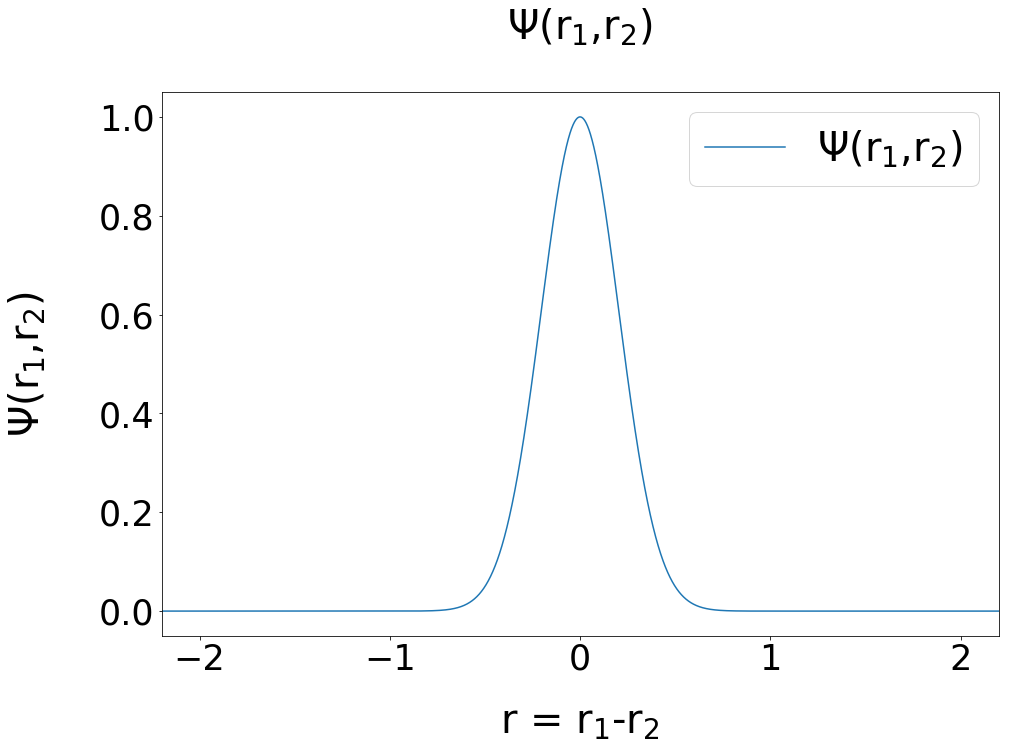
\includegraphics[width=\columnwidth]{Wavefunction.png}
	\caption{\label{wavefigure} The wave function of two electrons as the product of two 1s states. The function appears to have converged to zero at r = $\pm$1 for all practical purposes.}
\end{figure}
 The CPU time is estimated using the $WPI\_Wtime$ function. When the computation is preformed at each individual processor the function $WPI\_Reduce$ is applied to reassemble the result of the integral and variance estimates. Both the temporal efficiency and the accuracy for all three cases are evaluated and compared. The results are graphically represented in the result section, and tabulated values are located in the appendix. \\ \indent 
 Finally, the program is tested for $N=10^7$ using various compiler flags. The experiment is preformed 10 times per compiler flag \textit{-O1, -O2} and \textit{O3}. The time per compiler flag is then given as the average of all 10 runs. 
 
\section{Results}  \noindent
The ground state wave function for a two-electron system is plotted in figure \ref{wavefigure}. It is evident that the function is evenly distributed around zero with an exponentially decaying form. From a graphical evaluation the wave function appears to have converged to zero for $r = \pm 1$, for all practical purposes. $\lambda = \pm 3$ thus seams appropriate in order to leave a certain error margin. \\ \indent 
The main results of the Gauss-quadrature integration are presented in figure figure \ref{integrated_time_l} and \ref{integrated_results}. The tabulated values corresponding to the figures are presented in the appendix. It can be seen in figure \ref{integrated_time_l} that the Gauss-Laguerre procedure is more time costly than the simpler Gauss-Legendre method for all selected N values. The figure indicates that the logarithmic development of the time cost as a function of N grows at approximately the same rate, but with a different constant factor. That is, the cost of producing the Laguerre polynomials will rapidly become more expensive than the production of the Gauss-Legendre polynomials. The estimates are given for both Gauss-Legendre (represented by circles) and  Gauss-Laguerre (represented by triangles).
\begin{figure}[!hb]
	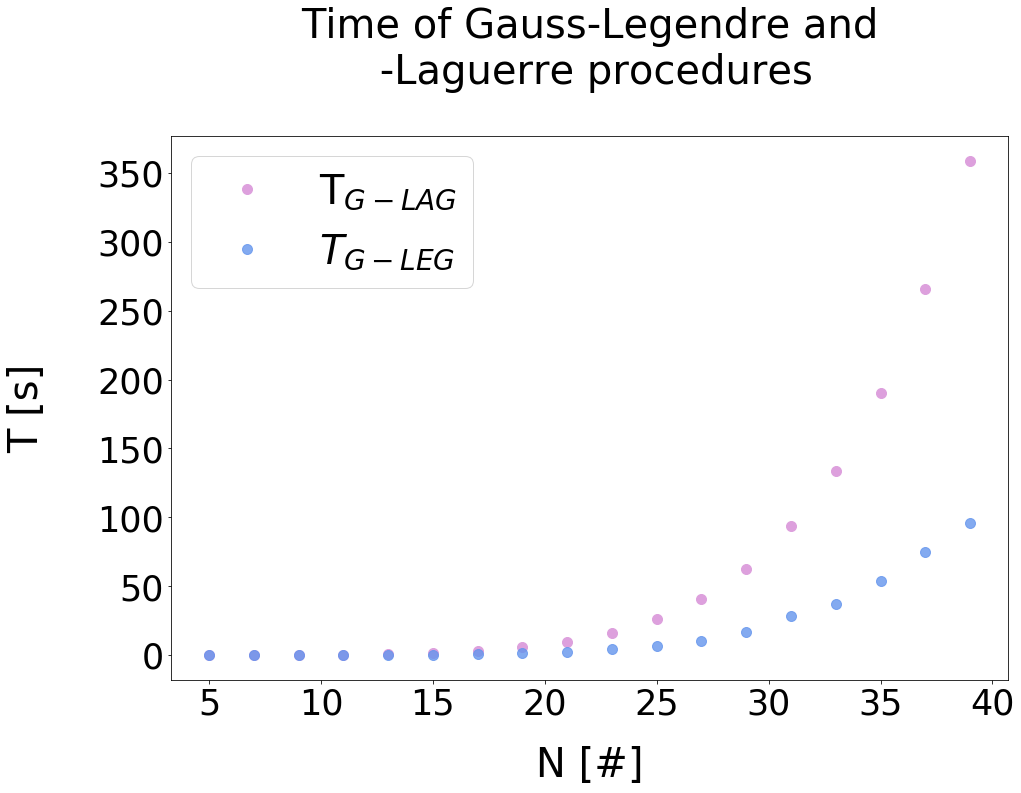
\includegraphics[width=\columnwidth]{Gauss_time.png}
	\caption{\label{integrated_time_l} The temporal result of the Gauss-Legendre and -Laguerre estimations of the correlation energy as a function of N in the log-space, based on 10 independent tests.}
\end{figure} 

\begin{figure*}[!ht]
	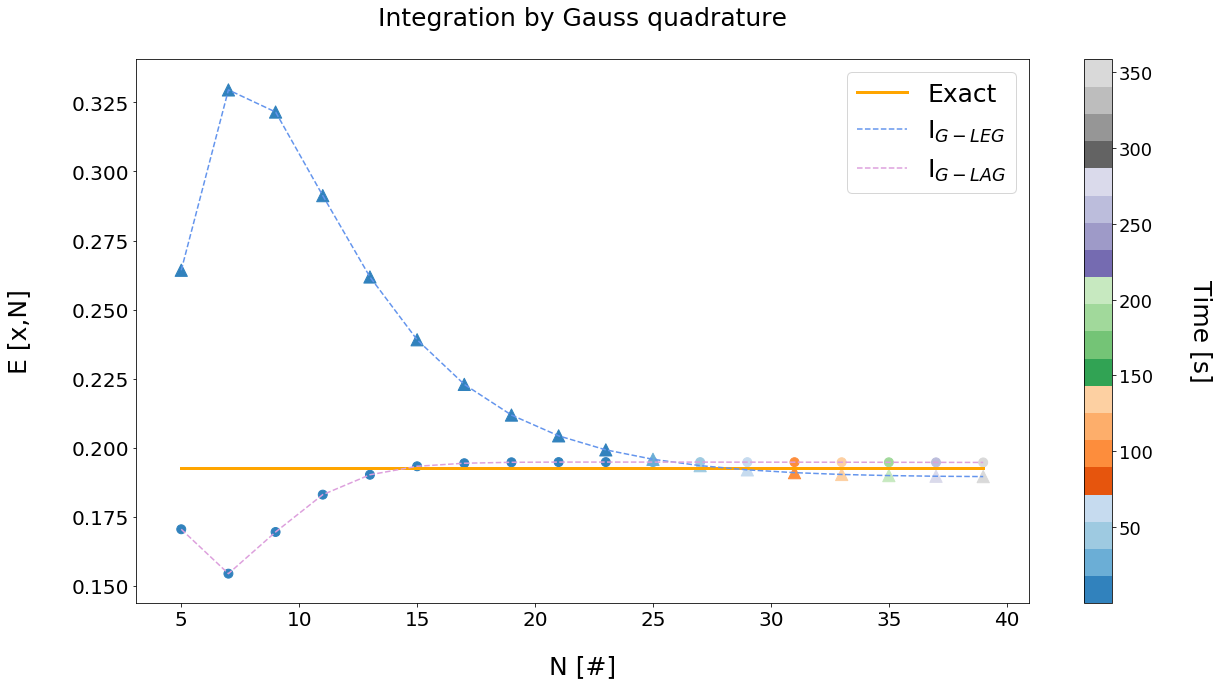
\includegraphics[scale = 0.4]{Gauss_lagleg_2.png}
	\caption{\label{integrated_results} The result of the Gauss-Legendre and Gauss-Laguerre procedures to approximate the expectation value for the interaction energy, as a function of N and the chosen x-range of $\lambda \in[-3,3]$. The exact result is $1.9277\times 10^{-1}$. \vspace{2cm}}
\end{figure*}
\noindent 
Figure 3 presents the correlation energy estimates as a function of N, and illustrates how the the Gaussian quadrature procedures converges. The tabulated values and a plot of the relative error are available in the appendix. From a graphical evaluation of figure \ref{integrated_results} it is evident that both procedures are converging towards approximately the closed form solution as N increases. The Legendre polynomials converges from above, while the Laguerre polynomials converge from below the closed form solution. What can also be seen is that the Legendre polynomials actually converges slightly below the closed form solution, while the Laguerre polynomials converges to value slightly above. The Laguerre polynomials appears to be the better approximation, and stabilizes earlier than the Legendre polynomials. That is, the former appears to have converged at N = 15 while the latter converges around N = 33. Thus, none of the polynomials ever fully reach the closed form solution with three leading digits for the selection of N values. The closest approximation is reached at N = 27 for the Gauss-Legendre polynomials with a value of $E[f] (1.9 \pm 0.2)\times 10^{-1}$, and $E[f]\approx (1.9 \pm 0.1)\times 10^{-1}$ through the Gauss-Laguerre polynomials. \newpage   \indent 
The expectation value of the correlation energy yielded by the Monte Carlo integration, as a function of N random samples, are presented in figure \ref{mc}. The brute force Monte Carlo integration $I_{MC}$, the importance sampled variance $I_{MC,IS}$ and the parallelized estimate $I_{MC, PAR}$ are represented, alongside the closed form solution value. Upon graphical evaluation of the plot it appears that the estimated energy converges towards the closed form solution as N increases by all three methods. The brute force Monte Carlo estimate is the one that appears to preform the poorest for lowest values of N, and appears to converge slower than the two improved methods. The unparalleled importance sampling appears to converge the fastest, at least for low values of N. Furthermore, for low values of N $I_{MC,IS}$ appears to yield the most accurate results. The best estimate is found for $N = 10^7$ with $E[f]\approx (1.8983 \pm 0.0003)\times 10^{-1}$ for $I_{MC}$,  $E[f]\approx (1.9292 \pm 0.0004)\times 10^{-1}$ for $I_{MC,IS}$ and $E[f]\approx (1.9264 \pm 0.0004)\times 10^{-1}$ for $I_{MC,PAR}$. The parallelized importance sampling is thus found to be the most accurate solution for a sufficiently large N, while $I_{MC,IS}$ is the most accurate for the lower values of N. 
\begin{figure}[H]
	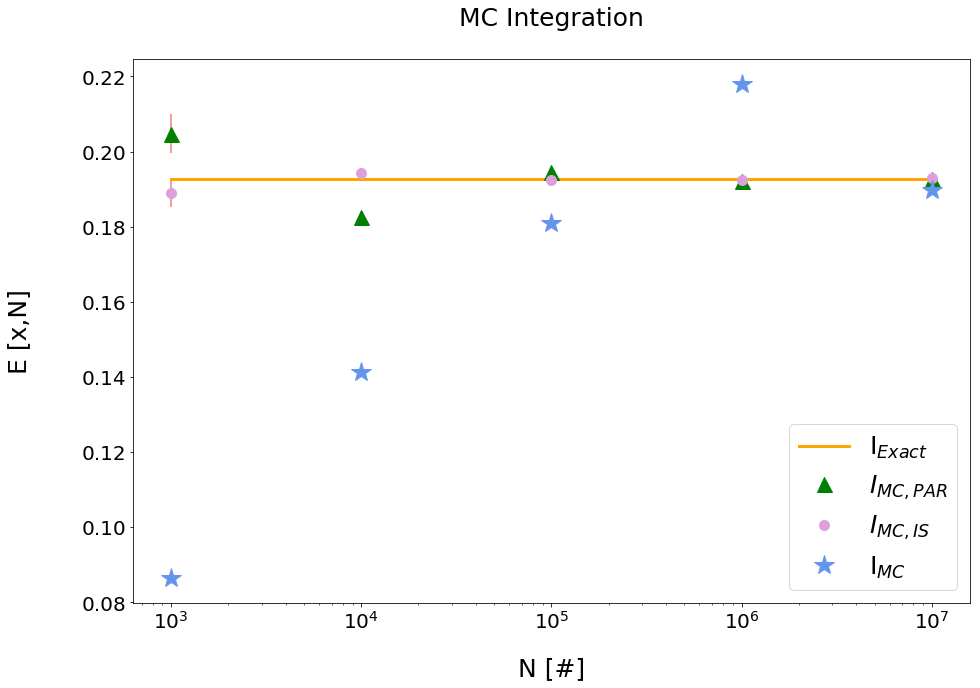
\includegraphics[width=\columnwidth]{MC_integration.png}
	\caption{\label{mc} The result of the Monte Carlo integration procedures to approximate the expectation value for the interaction energy, as a function of N and the chosen x-range of $\lambda \in[-3,3]$. The results from the brute force Monte Carlo are represented by the stars, the results from the importance sampling are represented by the circles and the parallelized results by the triangles. The exact result is $E[f] = 1.9277\times 10^{-1}$. }
\end{figure}
\begin{figure}[H]
	\vspace{34.3mm}
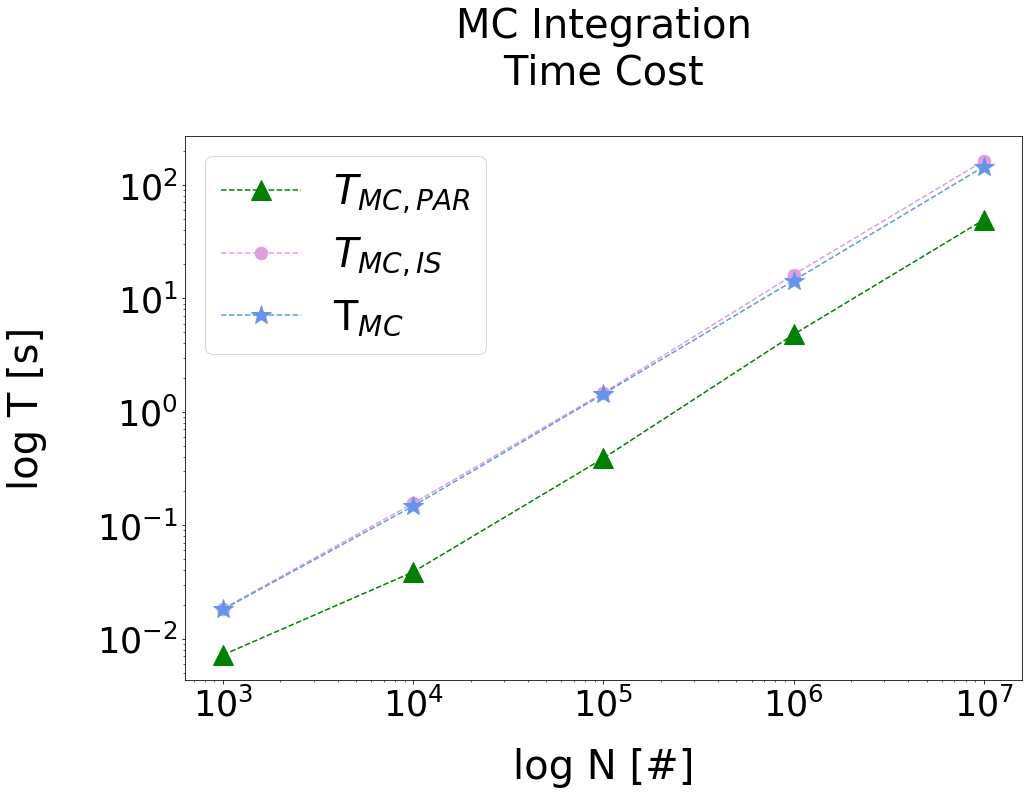
\includegraphics[width=\columnwidth]{MC_time.png}
\caption{\label{mc_time} The time cost of the Monte Carlo integration procedures to approximate the expectation value for the interaction energy, as a function of N and the chosen x-range of $\lambda \in[-3,3]$. The time cost of the brute force Monte Carlo are represented by the stars, the time cost of the importance sampling are represented by the circles and the parallelized time cost by the triangles.}
\end{figure} \newpage \noindent 
Figure \ref{mc_time} yields the time cost of each Monte Carlo procedure, while table \ref{time_mc_tab} shows the rates between the parallelized method with $I_{MC}$ and $I_{MC,IS}$. Looking at the plot it is evident that the time cost increases approximately linear in log-space. The time cost appears to be roughly the same for both $I_{MC}$ and $I_{MC,IS}$, but for the highest values of N one can see that $I_{MC,IS}$ becomes slightly more expensive than $I_{MC}$. The curve for $I_{MC,PAR}$ is shifted lower than $I_{MC}$ and $I_{MC,IS}$, and establishes that the parallelized version indeed reduces the time cost. Looking at the tabulated relative relations, it is apparent that this reduction is in the order of 2.5-4 times cheaper for $I_{MC,PAR}$. \\
Figure \ref{mc_err} presents the variation of the model as a function of N. It is evident that $I_{MC}$ has consistently the lowest variation as N increases, in the order of four leading digits accuracy. For both $I_{MC,PAR}$ and $I_{MC,IS}$ the variance decreases and converges towards zero as N increases at roughly the same rate. The parallelized Monte Carlo initially have the highest error, but reaches approximately the same value as the unparalleled importance sampling for $M \leq 10^4$. At $N=10^7$ all procedures have reached a predicted accuracy of four leading digits. \\ \indent
The average values of the compiler flag test are presented in table \ref{compilerflags}, with estimated variance of the 10 sample runs. The estimates all appears to be within each others variance range. \\

\begin{figure}[H]
		\vspace{16mm}
	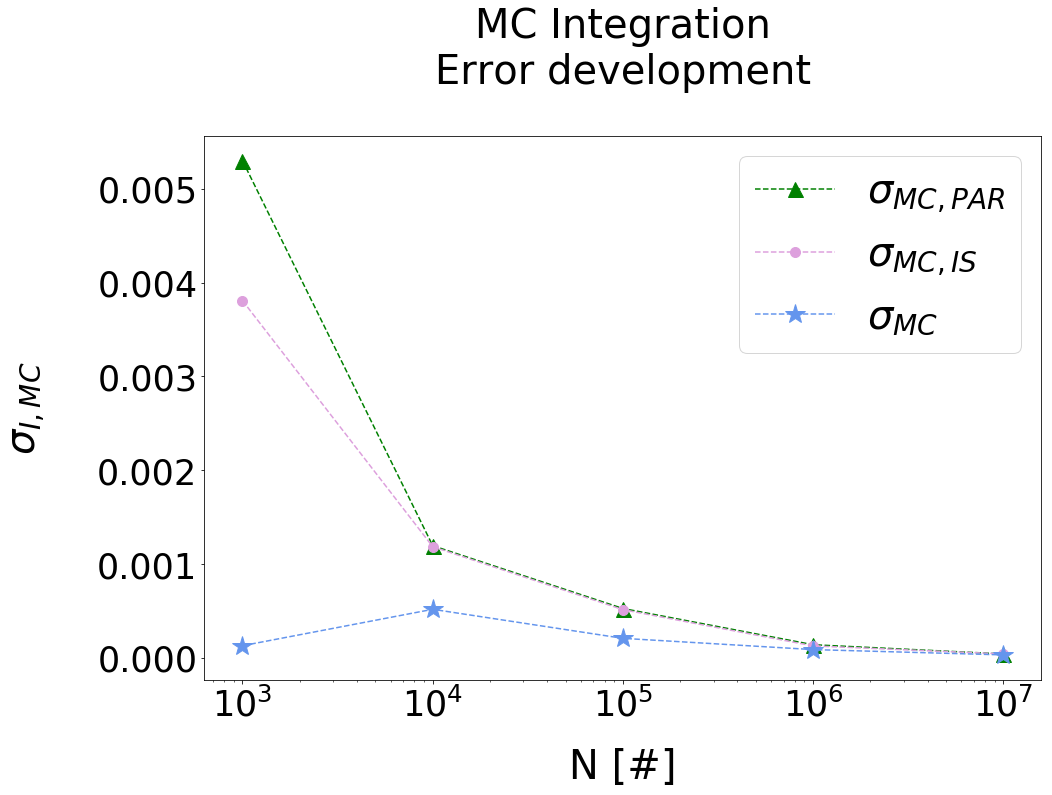
\includegraphics[width=\columnwidth]{MC_integration_error.png}
	\caption{\label{mc_err} The error of the Monte Carlo integration procedures to approximate the expectation value for the interaction energy, as a function of N and the chosen x-range of $\lambda \in[-3,3]$. The error for the brute force Monte Carlo are represented by the stars, the error of the importance sampling are represented by the circles and the parallelized errors by the triangles.}
\end{figure} 
\newpage 
\begin{table}[H]
	\caption{\label{time_mc_tab} The time rate averages of N samples of the parallelized mc integration weighted in regards to the brute force and importance sampling procedures.}
	\centering 
	\begin{tabular}{|c|c|c|}
		\hline 
		\hspace{1mm}\textbf{N} \hspace{1mm}& \hspace{1mm} \textbf{MC/MC$_{par}$} \hspace{1mm} & \hspace{1mm}\textbf{MC$_{IS}$/MC$_{PAR}$} \hspace{1mm} \\ \hline 
10$^3$ & 3.9730  & 3.9160  \\
10$^4$ & 2.6282  & 2.4859  \\
10$^5$ & 2.7132  & 2.6479  \\
10$^6$ & 3.3489  & 2.9734  \\
10$^5$ & 3.4015  & 3.0224  \\
		\hline 
	\end{tabular} \\ 
\end{table}

\begin{table}[H]
	\caption{ \label{compilerflags} The time cost of using various compiler flags tested at $N = 10^7$.}
	\centering 
	\begin{tabular}{|c|c|c|}
		\hline 
		\hspace{1mm} \textbf{Compiler Flag} \hspace{1mm} & \hspace{1mm}\textbf{Average time [s]} \hspace{1mm} & \textbf{Variance [s]} \\ \hline 
		O1& 50.0450 &0.7286 \\
		O2& 49.8718 &2.9312 \\ 
		O3& 50.9497 & 1.7525\\
		\hline 
	\end{tabular} 
\end{table}

\twocolumngrid


\section{Discussion} \noindent 
In regards to the chosen $\pm \lambda$ integration limits, the choice and results appears reasonable. A way to investigate the effect of the choice of $\lambda$ would of course be to evaluate the integral while varying $\lambda$, and then look at the effect the altercation would have on the estimate. This is although deemed excessive for the purpose of this paper, and is left for future work. \\ \indent 
Looking at the results for the Gauss-Legendre and Gauss-Laguerre polynomials it is hard to say why the two procedures end up converging towards slightly offset values. It might be due to an error in the implementation, or it might be a methodical fault.  Given that both the Gauss-Legendre and Gauss-Laguerre are very thoroughly understood and fairly straight forward procedures it appears very unlikely that it is due to a methodical error. The background implementation functions provided for the above procedures are rather unclear. It could easily lead to a misunderstanding in further implementations or possibly contain errors. Perhaps in the some of the hard coded values found in the code that is hard to test. The evaluation of the source of this error is left for future work, but it should be noted that this error is particularly interesting as the estimate converges wrong in both cases of the quadrature. This might be an indication of an implementation fault. \\ \indent
The other main result for the quadratures stated that time cost of both procedures were linear in log-space. This is an indication that both procedures are subjected to a power law, that likely could be found fitting a line to the curves. It is interesting to see that the slopes of the methods appears parallel, and only differentiates by a constant factor. The evaluation of the power laws are left for further work, and a clarification of why the slopes appears to be equal would probably involve a detour into the mathematical foundation of the polynomials. It is no surprise that an increase in N increases the time cost of the estimation in general, as it would imply an increase in the number of floating point operations necessary to complete the procedure. The results appear reasonable in this aspect. \\ \indent 
Regarding the error estimates of the quadratures, it should be stated that it is probable that the real accuracy  of the estimates is a lot higher than what is indicated by looking at the relative error. This is supported by the fact that for sufficiently high N the actual difference between the estimate and the closed form solution are a significant factor lower than what the relative error indicates. Furthermore, for low values of N the error estimate does not even appear to make sense. For the highest values of N, the large relative error would also be partly caused by the fact that the estimate converges to the wrong value. It does indeed exist more suitable error analysis for numerical integrations over the Gauss Quadrature, like for instance the procedures outlined by R. Z. Iqbal and M.O. Ahmed \footnote{Error Estimation of Numerical Integration Methods, Department of Mathematics and statistics, University of Lahore, Pakistan, 2016}. or by F. G. Lether \footnote{Error estimates for Gaussian quadrature, AMC 1980}. \\ \indent 
In regards to the Monte Carlo integration methods, everything appears more in accordance to what one would expect. The importance sampling does indeed increase the accuracy for the particular choice of N in all regards. This makes sense, as focusing only on the relevant values of abscissas would imply a a higher relevancy value for each sample N. In some sense, some of the less efficient data dragging up the time cost is discharged. This of course would have the larges effect on the lowest value of N, as the results would be sensitive to the choice of abscissas when the abscissas are few. This is evident in the results, and the estimates appears reasonable. That the parallelized importance sampling estimate has a lower value than the importance sampling itself also makes sense for low N. For a low value of N, each processor rapidly gets very few abscissas to work with as it only works on N/4 samples. This would not have the same effect for higher N, as at a certain threshold the solution would have properly converged anyhow for each individual processor. \\ \indent 
Looking at the time cost estimates for the Monte Carlo procedures we see that up until a rather large value for N, the importance sampling procedure does not cost much more than the brute force Monte Carlo. It appears therefore to be a rather cheap improvement with a high value gain in accuracy. As expected, when the procedure is parallelized the time cost goes significantly down. It appears to be approximately 4 times cheaper than the unparalleled procedure. This is sensible as the procedure was run using 4 times the processors simultaneously.\\ \indent 
In regards to the error estimates we see for all variations of procedures that $\sigma$ decreases as N increases. The accuracy becomes better the more abscissas one samples, which is sensible. If it was possible to find a more suitable error measurement than the relative error for the Gauss Quadrature, it would perhaps be easier to compare the two methods. \\ \indent 
Looking solely at the Monte Carlo integrations, we find that the variation estimates with the highest precision is the brute force Monte Carlo. This is not completely reasonable, because the closed form solution is not within the range of the variance for any of brute force estimations. The evaluation of why this is is left for future work. That the parallelized code yields a slightly higher variation than the one that is not parallelized is unsurprising for the same reason as states above. 
\newpage 
\section{Conclusion} \noindent 
In this paper we have estimated the expectation value of the correlation energy between two electrons in an helium atom, using Gaussian Quadrature and Monte Carlo Integration. In general, it was established that a higher accuracy in the result was achieved by increasing N, at the price of a time cost. \\ \indent For $N<39$, it was found that the best estimate produced by th Gauss-Legendre procedure was $E[f] \approx (1.9 \pm 0.2)\times 10^{-1}$ for $N=27$. The best estimate for the Gauss-Laguerre procedure was found to be $E[f]\approx (1.9 \pm 0.1)\times 10^{-1}$ for $N=15$, testes for the same range of N. The error estimate was found slightly high in both cases, due to the method of error estimation. The best result from brute force Monte Carlo integration using a uniform distribution function was estimated for $N=10^7$ yielding $E[f]\approx (1.8983 \pm 0.0003)\times 10^{-1}$. The importance sampling procedure improved this result and estimated $E[f]\approx (1.9292 \pm 0.0004)\times 10^{-1}$ for $N=10^7$. The estimation was acknowledged as better in the case of the Monte Carlo integration, as the variation estimate yielded a much higher precision than the Gaussian Quadrature. The code was furthermore parallelized, yielding an estimate of approximately the same accuracy, resulting in $E[f]\approx (1.9264 \pm 0.0004)\times 10^{-1}$.\\ \indent 
Throughout this paper we have thus explored some of the challenges and predictions of two well established methods for numerical integration. Based on a rather poor approach to evaluating the accuracy of the Gauss Quadrature, it was found hard to compare the two methods. If one although should state anything on the basis of these results, the parallelized importance sampling from the Monte Carlo integration would indeed be the best approach to the closed form solution. This is stated both due to the result having the highest accuracy, and because it were the least time costly. In total the project is found successful in its evaluation of the procedures, but a comparison of the methods could benefit a lot from a better understanding of the errors. Furthermore, as with any experiment the estimates could also benefit from an increased number of test to yield a more solid foundation for the results. 

\newpage. \newpage
\onecolumngrid
\section{Referances}
[1] Handbook of computational methods for integration, P. K. Kythe and M. R. Schaferkotter, Chapman \& Hall/CRC, Boca Raton Florida, 2005.\\

[2] Numerical recipes, M. W. Pratt et al, 2rd edition, Cambridge university press, 2007.\\  

[3] M. H. Jensen, Computational physics lecture notes, Department of Physics university of Oslo, 2015. \\

[4] K. Rottman, Matematisk formelsamling, Spektrum forlag, 2017
\newpage 
\section{Appendix}
\subsection{Tabulated values}

\begin{table}[!h]
	\caption {Gauss-Legendre Quadrature. \label{legendre_values} \centering  Integrated expectation value estimate using Gauss-Legendre quadrature. The error estimate is given as the relative error.} 
	\begin{tabular}{|c|c|c|c|}
		\hline 
		\hspace{5mm} \textbf{N} \hspace{5mm} & \textbf{Integrated value $\times 10^{-1}$} & \hspace{3mm}\textbf{Relative error $\times 10^{-1}$} & \hspace{3mm}\textbf{Time  [s]} \hspace{5mm}\\
		\hline 
			5 & 2.642  & 4  & 0.0009 \\
			7 & 3.295  & 7  & 0.0063 \\
			9 & 3.215  & 7  & 0.0218 \\
			11 & 2.913  & 5  & 0.0572 \\
			13 & 2.618  & 3  & 0.1633 \\
			15 & 2.391  & 2  & 0.3104 \\
			17 & 2.229  & 2  & 0.6593 \\
			19 & 2.118  & 1  & 1.3405 \\
			21 & 2.043  & 0.6  & 2.4468 \\
			23 & 1.992  & 0.3  & 4.1460 \\
			25 & 1.958  & 0.2  & 6.5590 \\
			27 & 1.935  & 0.04  & 10.4028 \\
			29 & 1.920  & 0.04  & 16.5082 \\
			31 & 1.910  & 0.09  & 28.1410 \\
			33 & 1.903  & 0.1  & 37.0551 \\
			35 & 1.899  & 0.1  & 53.6300 \\
			37 & 1.897  & 0.2  & 74.8152 \\
			39 & 1.896  & 0.2  & 95.8025 \\

		\hline 
	\end{tabular} 
\end{table}

\begin{table}[!h]
	\caption{Gauss-Laguerre Quadrature. \label{laguerre_values} \centering Integrated expectation value estimate using Gauss-Laguerre quadrature. The error estimate is given as the relative error.}
	\begin{tabular}{|c|c|c|c|}
		\hline 
		\hspace{5mm} \textbf{N} \hspace{5mm} & \textbf{Integrated value} $\times 10^{-1}$ & \textbf{Relative Error} $\times 10^{-1}$ & \hspace{3mm}\textbf{Time  [s]} \hspace{5mm}\\
		\hline 
			5 & 1.7049  & 1  & 0.0057 \\
			7 & 1.5442  & 2  & 0.0293 \\
			9 & 1.6950  & 1  & 0.1112 \\
			11 & 1.8302  & 0.5  & 0.2725 \\
			13 & 1.9022  & 0.1  & 0.6307 \\
			15 & 1.9328  & 0.03  & 1.5614 \\
			17 & 1.9440  & 0.09  & 3.2090 \\
			19 & 1.9473  & 0.1  & 6.2235 \\
			21 & 1.9481  & 0.1  & 9.6838 \\
			23 & 1.9481  & 0.1  & 16.1813 \\
			25 & 1.9480  & 0.1  & 25.9065 \\
			27 & 1.9480  & 0.1  & 40.4221 \\
			29 & 1.9478  & 0.1  & 62.5119 \\
			31 & 1.9477  & 0.1  & 93.3598 \\
			33 & 1.9476  & 0.1  & 133.3770 \\
			35 & 1.9473  & 0.1  & 190.5940 \\
			37 & 1.9471  & 0.1  & 265.4100 \\
			39 & 1.9468  & 0.1  & 358.7210 \\

		
		\hline 
	\end{tabular}
\end{table}

\newpage 

\begin{table}[!h]
	\caption{Brute force Monte Carlo integration. 	\label{mc_values} \centering The integrated value of the system using Monte Carlo integration. The values are the averages of 10 independent runs of the procedure. }
	\begin{tabular}{|c|c|c|c|}
		\hline 
		\hspace{5mm} \textbf{N} \hspace{5mm} & \textbf{Integrated value} $\times 10^{-1}$& \hspace{3mm} \textbf{Variance} $\times 10^{-1}$ & \hspace{3mm} \textbf{Time  [s]} \hspace{5mm}\\
		\hline 
			10$^3$ & 0.8657  & 0.0013  & 0.0181 \\
			10$^4$  & 1.4134  & 0.0052  & 0.1476 \\
			10$^5$  & 1.8097  & 0.0021  & 1.4372 \\
			10$^6$  & 2.1790  & 0.0009  & 14.3547 \\
			10$^7$  & 1.8983  & 0.0003  & 145.0928 \\
		\hline 
	\end{tabular}
\end{table}


\begin{table}[!h]
	\caption{Monte Carlo Importance Sampling. \label{mc_values_is} \centering The integrated value of the system using Monte Carlo integration with importance sampling. The values are the averages of 10 independent runs of the procedure.}
	\begin{tabular}{|c|c|c|c|}
		\hline 
		\hspace{5mm} \textbf{N} \hspace{5mm} & \textbf{Integrated value} $\times 10^{-1}$& \hspace{3mm} \textbf{Variance}  $\times 10^{-1}$& \hspace{3mm} \textbf{Time  [s]} \hspace{5mm}\\
		\hline 
			10$^3$ & 1.8901  & 0.0381  & 0.0184 \\
			10$^4$ & 1.9440  & 0.0118  & 0.1561 \\
			10$^5$ & 1.9231  & 0.0051  & 1.4726 \\
			10$^6$ & 1.9254  & 0.0013  & 16.1675 \\
			10$^7$ & 1.9292  & 0.0004  & 163.2929 \\

		\hline 
	\end{tabular}
\end{table}


\begin{table}[!h]
	\caption{Monte Carlo Parallelized Importance Sampling. 	\label{mc_values_par} \centering The integrated value of the system using Monte Carlo integration with importance sampling and parallelization The values are the averages of 10 independent runs of the procedure. }
	\begin{tabular}{|c|c|c|c|}
		\hline 
		\hspace{5mm} \textbf{N} \hspace{5mm} & \textbf{Integrated value}$\times 10^{-1}$ & \hspace{3mm} \textbf{Variance} $\times 10^{-1}$ & \hspace{3mm} \textbf{Time  [s]} \hspace{5mm}\\
		\hline 
			10$^3$ & 2.0479  & 0.0530  & 0.0072 \\
			10$^4$ & 1.8259  & 0.0120  & 0.0388 \\
			10$^5$ & 1.9457  & 0.0053  & 0.3899 \\
			10$^7$ & 1.9222  & 0.0014  & 4.8073 \\
			10$^8$ & 1.9264  & 0.0004  & 49.3534 \\
		\hline 
	\end{tabular}
\end{table}
\begin{figure}[H]
	\centering
	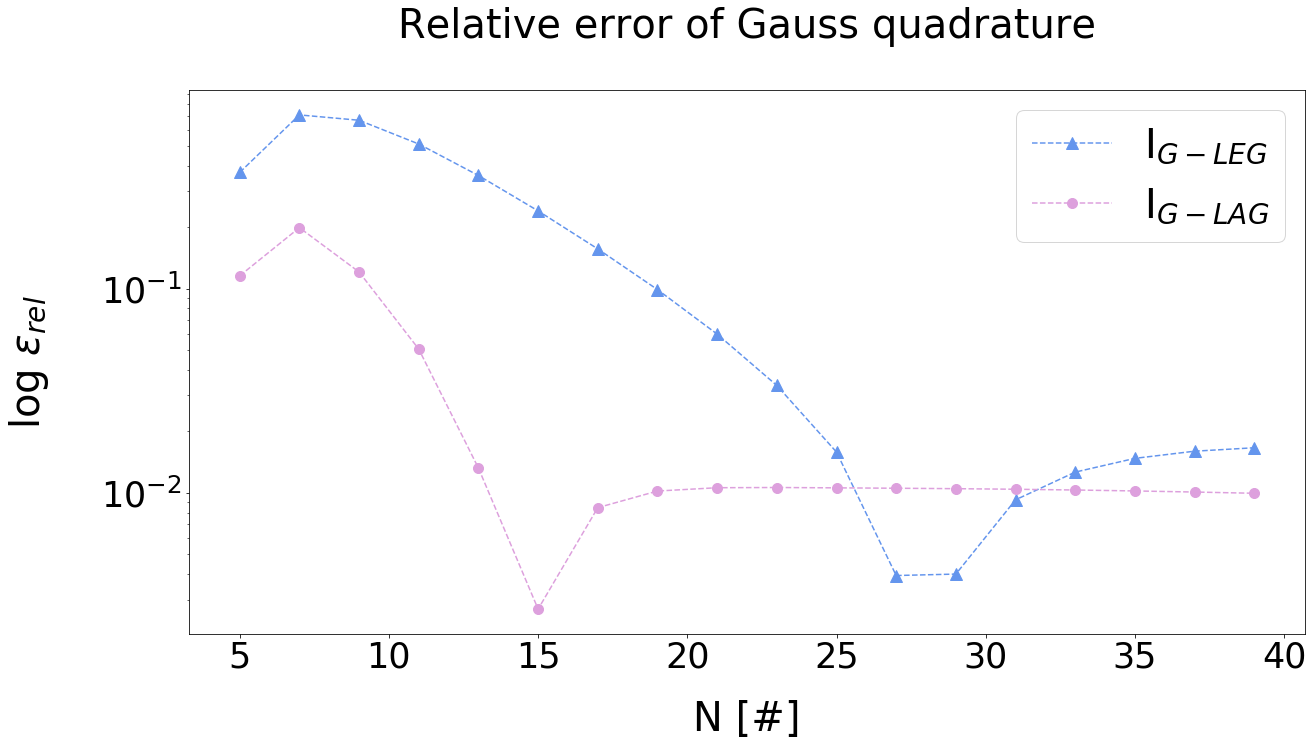
\includegraphics[scale = 0.3]{Gauss_lagleg_err.png}
	\caption{\label{laglegerr} The log-space of the relative error in the Gaussian Quadrature procedures.}
\end{figure} \newpage 

\subsection{Derivation of analytical value}\noindent 
To find the ground state expectation value for the correlation energy between two electrons in a Helium atom, i.e. $\alpha = 2$, one can start with equation \ref{ccintegration} and rewrite the expression to spherical coordinates. Applying equation \ref{r12} and \ref{r1r2}, and begin with the integral dependent on $\mathbf{r}_2$ \vspace{2mm}\\ 
\begin{equation*}
	I = \int \dfrac{e^{-2\alpha r_2}}{\abs{\mathbf{r_1}-\mathbf{r_2}}}d^3\mathbf{r}_2 = \int \dfrac{e^{-2\alpha r_2}}{\sqrt{r_1^2+r_2^2-2r_1r_2\cos\theta_2}}r_2^2\sin\theta_2dr_2d\theta_2d\phi_2 
\end{equation*}\vspace{4mm}\\ 
The $\theta$-dependent integral yields\vspace{2mm}\\ 
\begin{align*}
	\int_{0}^{max}\dfrac{\sin\theta_2}{\sqrt{r_1^2+r_2^2-2r_1r_2\cos\theta_2}}d\theta_2 = \dfrac{\sqrt{r_1^2+r_2^2-2r_1r_2\cos\theta_2}}{r_1r_2} \bigg|_0^\pi \\ \\ 
	= \dfrac{1}{r_1r_2}\qty(\sqrt{r_1^2+r_2^2 + 2r_1r_2} - \sqrt{r_1^2+r_2^2 -2r_1r_2})
	= \dfrac{1}{r_1r_2}\qty[(r_1+r_2)-\abs{r_1-r_2}]\\ \\
	= 	 \left\{
	\begin{array}{ll}
	2/r_1 & \textnormal{ if } r_2 < r_2\\
	2/r_2 & \textnormal{ if } r_2 > r_2
	\end{array} \right\} \\ 
\end{align*}\vspace{2mm}\\ 
The $\phi$ integral will be trivial and\vspace{2mm}\\ 
\begin{equation*}
	\int_{0}^{2\pi}d\phi = 2\phi
\end{equation*}\vspace{2mm}\\ 
So the entire integral becomes \vspace{2mm}\\ 
\begin{align*}
	I = 4\pi\qty(\dfrac{1}{r_1}\int_{0}^{r_1}e^{-2\alpha r_2}r_2^2dr_2 + \int_{r_1}^{\infty}e^{-2\alpha r_2}dr_2) \\  \\
	= \dfrac{\pi a^3}{8r_1}\qty[1-(1+\dfrac{2r_1}{a})e^{-2\alpha r_1}]
\end{align*}\vspace{2mm}\\ 
By repeating the exact same procedure for the integral over $r_1$, one obtains\vspace{2mm}\\ 
\begin{align*}
	(\dfrac{e^2}{4\pi\epsilon_0})\qty(\dfrac{8}{\pi a^3})\int\qty[1-(1+\dfrac{2r_1}{a})e^{-2\alpha r_1}]e^{-2\alpha r_1}r_1sin\theta_1dr_1d\theta_1d\phi_1
\end{align*}\vspace{2mm}\\ 
Applying $a=\pi$\vspace{2mm}\\ 
\begin{equation*}
	\int_{0}^{\infty}\qty[re^{-2\alpha r}-\qty(r+\dfrac{2r^2}{a})e^{-8r/2}]dr = \dfrac{5a^2}{16^2} = \dfrac{5\pi^2}{16^2}
\end{equation*}
\end{document}